\section{ドキュメントの構成}
作成したドキュメントの構成は以下の要素から構成されている. 
また, 作成にあたってROS WikiのNavigationページを参考にした.
\cite{ros_wiki_navigation}
\begin{itemize}
     \item \textbf{自己位置推定(AMCL)}
     \begin{itemize}
        \item \textbf{最低限の設定}
        \item \textbf{主要パラメータの調整}
        \item \textbf{その他パラメータの調整}
        \item \textbf{ROS\_ERRORが出たときの問題と対処法}
    \end{itemize}
     \item \textbf{経路計画(Move Base)}
    \begin{itemize}
        \item \textbf{最低限の設定}
        \item \textbf{Move Baseの土台となるパラメータ調整}
        \item \textbf{リカバリ動作のパラメータ調整}
        \item \textbf{コストマップのパラメータ調整}
        \item \textbf{ローカルプランナーのパラメータ調整}
        \item \textbf{グローバルプランナーのパラメータ調整}
        \item \textbf{ROS\_WARNが出たときの問題と対処法}
    \end{itemize}
\newpage
     \item \textbf{地図}
    \begin{itemize}
        \item \textbf{地図作成方法の説明}
        \item \textbf{slam\_toolboxでの地図作成方法}
        \item \textbf{glimでの地図作成方法}
    \end{itemize}
    \item \textbf{オドメトリ}
    \begin{itemize}
        \item \textbf{オドメトリの調整手順}
    \end{itemize}     
\end{itemize}

\section{ドキュメントの例示}
本論文では, 作成したドキュメントの中から例示として, オドメトリ調整と自己位置推定(AMCL)の
2項目を取り上げ, 記載内容の一部を示す. 

\subsection{オドメトリ調整}
調整対象のパラメータは, 車輪半径に関する補正係数であるwheel\_radius\_multiplierと, 車輪環距離に関する補正係数であるwheel\_separation\_multiplierの2つである. 
これらはロボットのオドメトリの正確さに直結するため, 自己位置推定を行う上で最初に調整すべき項目である. 

調整手順は以下の通りである. まず, Rvizを用いてトピックの可視化の準備を行う. 固定座標系をodomに設定し, LaserScanトピックを表示することで, ロボットの移動に伴うセンサ計測をできるようにする. 

次に, ロボットを壁から数メートル離れた位置に配置し, 直進させて並進成分の正確さを確認する. 
このとき, 得られるレーザスキャンに厚みが生じる場合は, wheel\_radius\_multiplierを調整する. 

さらに, ロボットをその場で回転させ, 回転成分の正確さを確認する. 
スキャンが1〜2度以上ずれている場合は, wheel\_separation\_multiplierを調整する. 
最後に再度直進させ, 並進と回転の双方でスキャンが一致していることを確認した時点で調整を完了とする. 

\figref{fig:Scanvisualizedinrviz}にオドメトリ調整前後のレーザスキャンをRvizで可視化した様子を示す. 
\begin{figure}[h]
     \centering
     \begin{minipage}[c]{65mm}
         \centering
         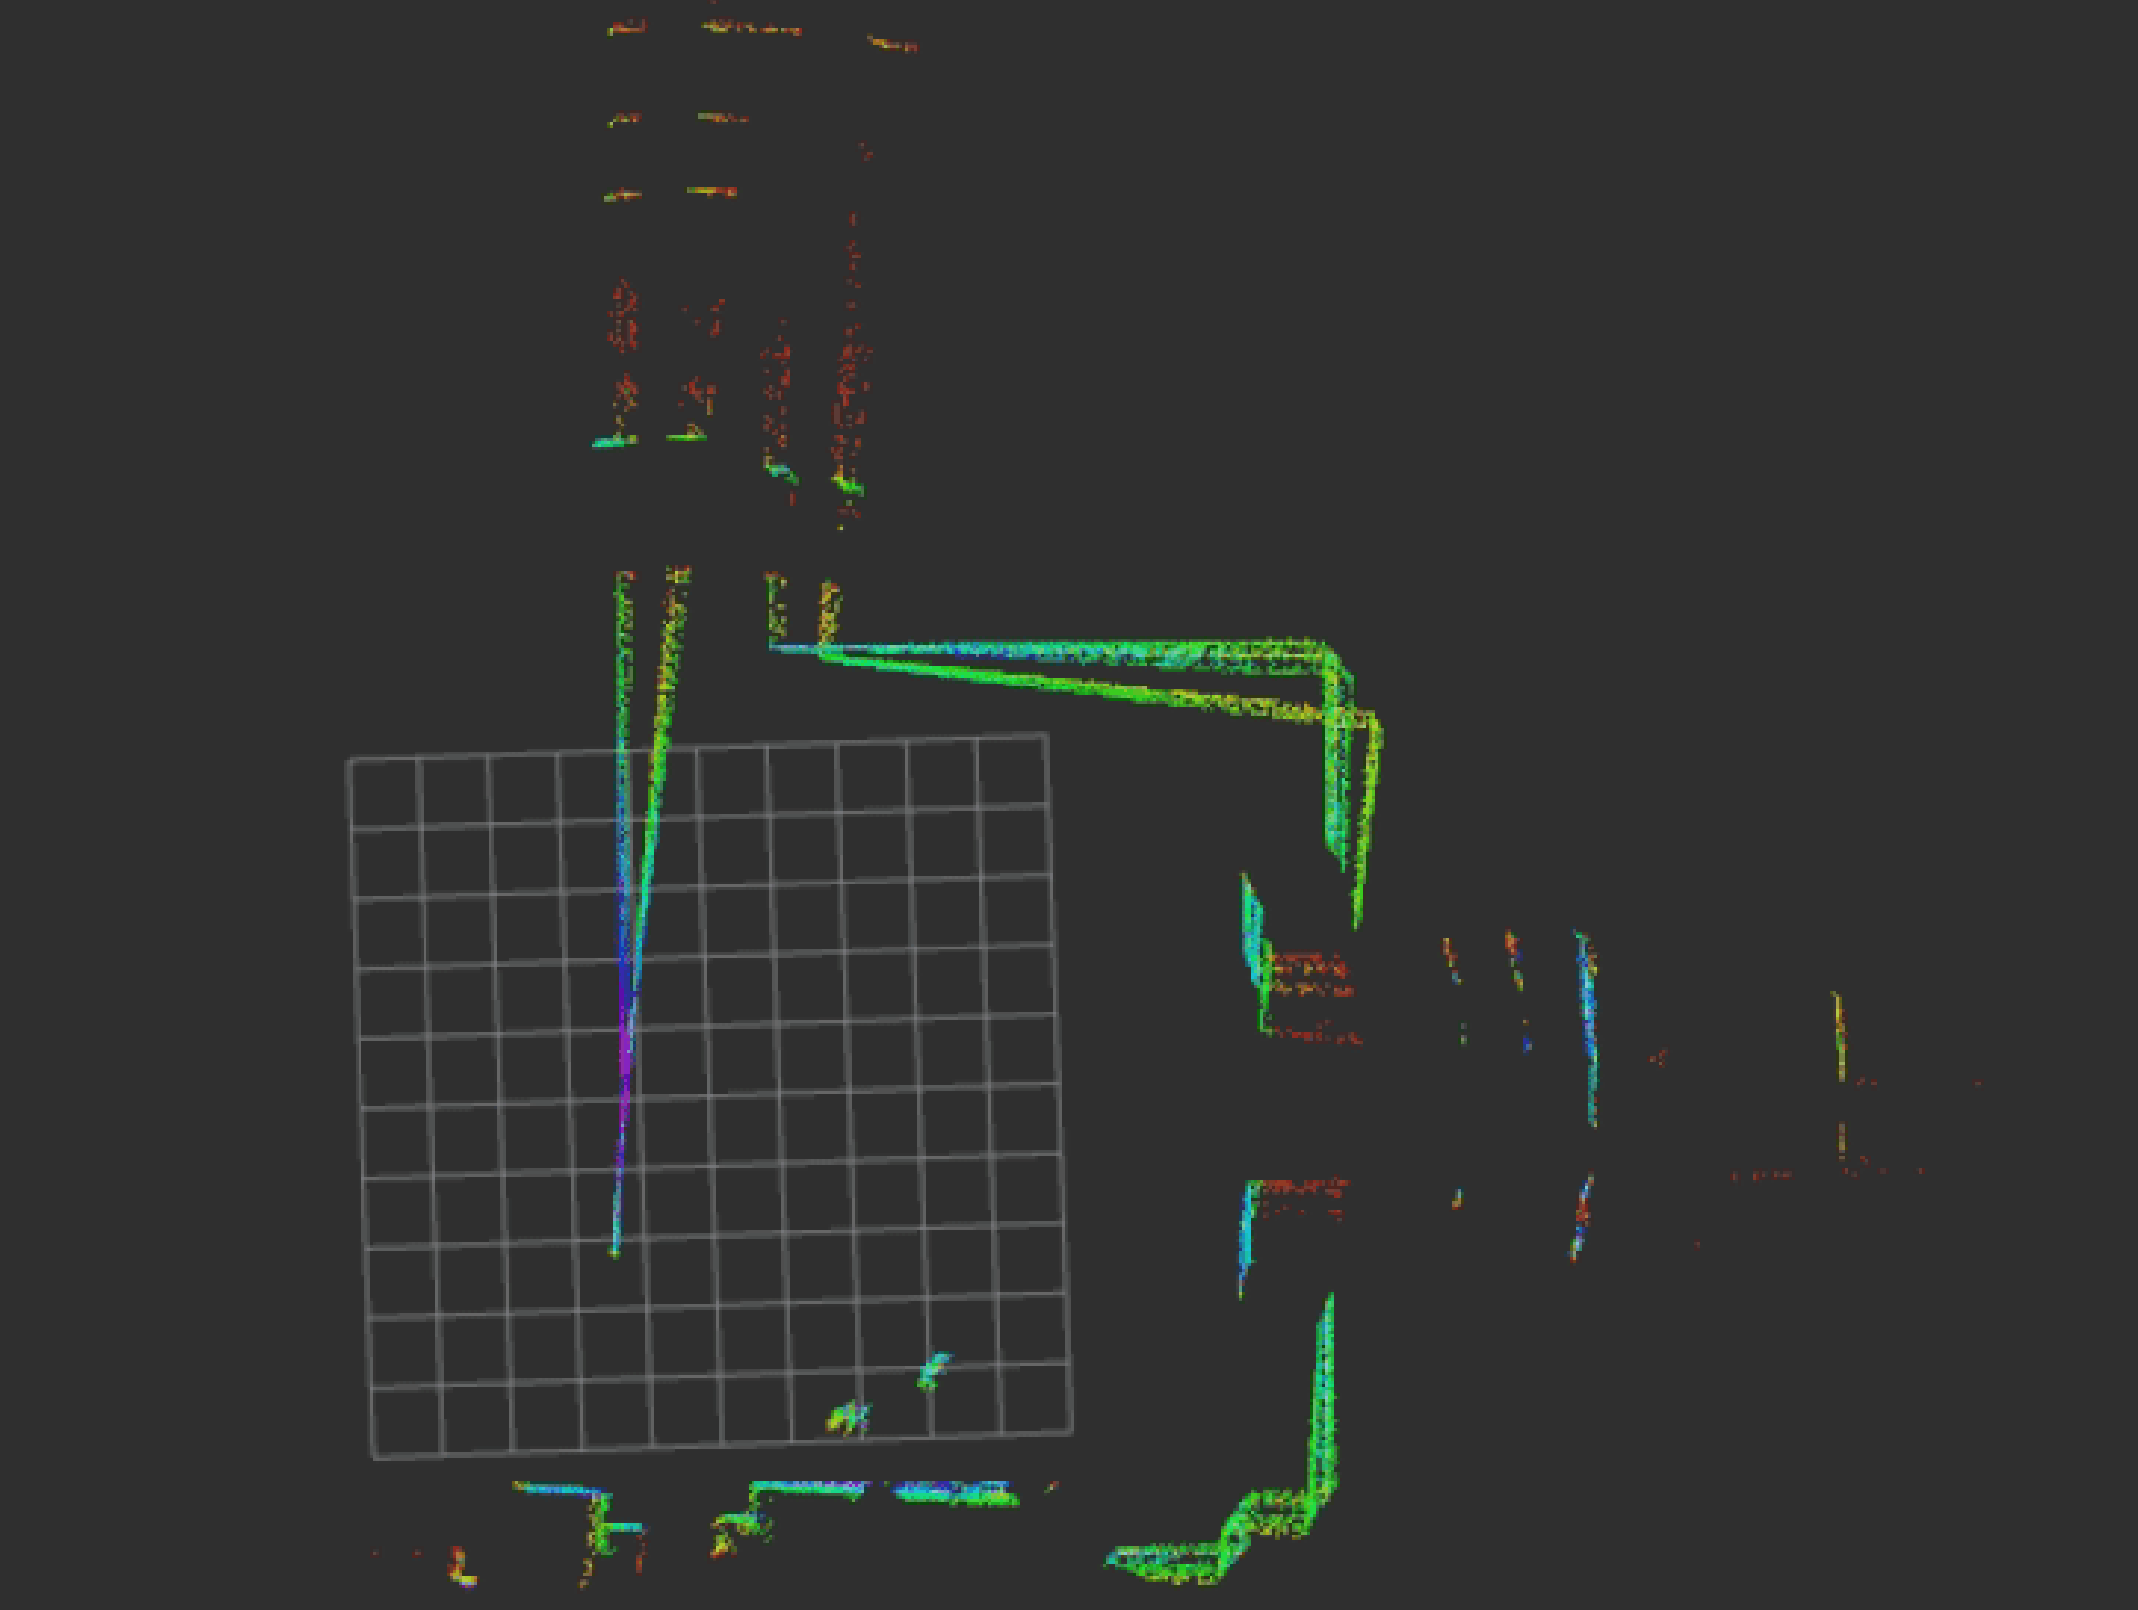
\includegraphics[height=40mm]{images/before_odom.png}
         \subcaption{Before odometry adjustment}
     \end{minipage}
     \begin{minipage}[c]{65mm}
         \centering
         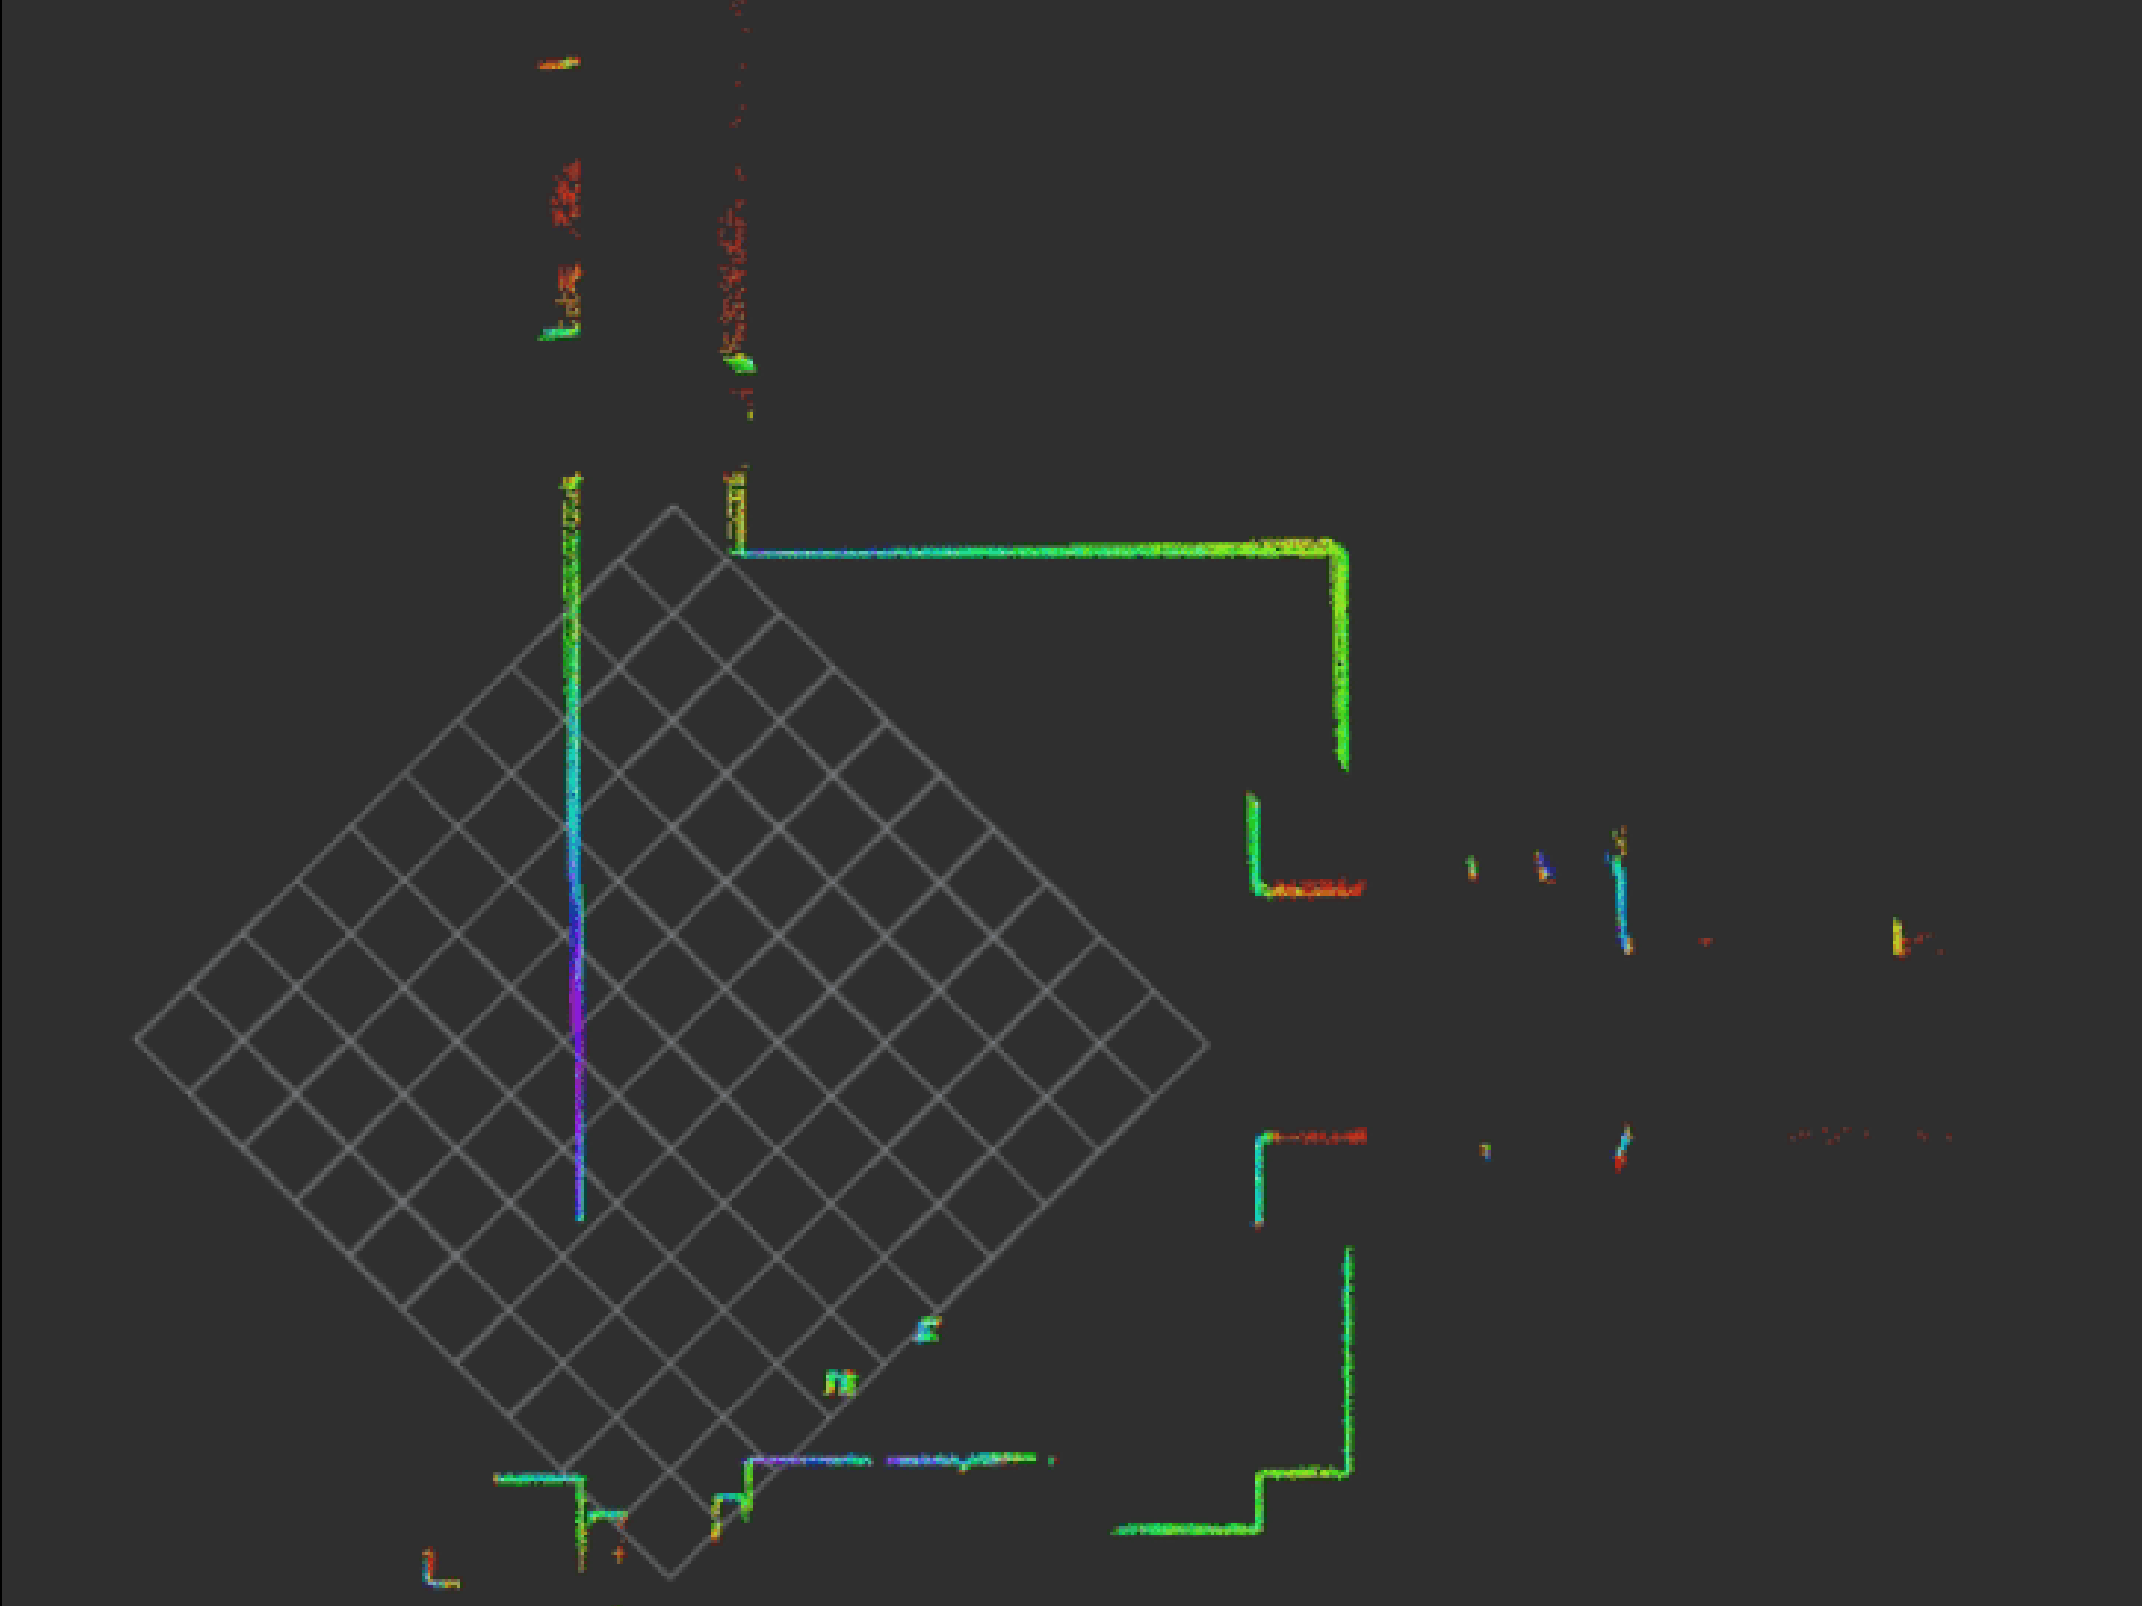
\includegraphics[height=40mm]{images/after_odom.png}
         \subcaption{After odometry adjustment}
     \end{minipage}
     \caption{Scan visualized in Rviz}
     \label{fig:Scanvisualizedinrviz}
\end{figure}

\subsection{AMCLにおけるオドメトリ関連パラメータの調整}
自己位置推定に用いるAMCLにおいて, 最初に調整すべきパラメータはodom\_alpha1〜odom\_alpha4である. 
これらはオドメトリの信頼度を決定する値であり, 大きな値を設定すると, オドメトリに含まれるノイズが大きいとみなされ, オドメトリの影響が小さくなる. 
一方で, 小さな値を設定するとオドメトリを強く信頼するようになる. 屋外環境ではオドメトリ誤差が大きくなるため, パラメータを過度に小さくすると誤推定に繋がる危険がある. 
特にodom\_alpha2とodom\_alpha3の調整が有効である. 

調整方法は以下の通りである. まず, 走行データをrosbagで記録し, Rvizを用いてパーティクルの散らばりや自己位置のずれ方を可視化する. 
これにより, どのパラメータが問題に寄与しているかを予測できる. その後, 記録したデータを再生し, パラメータを変更しながらオフラインでAMCLを動作させることで, パーティクルの挙動を確認できる. 

調整の基準としては, スキャンデータと地図の対応関係を利用する. 例えば, スキャンが並進方向にずれる場合はodom\_alpha3を増加させることで改善できる. 
また, 回転方向にずれる場合はodom\_alpha2を増加させることで修正を試みる. 
自己位置が徐々にずれていく場合には, odom\_alpha1〜odom\_alpha4させることで安定化を図る. 
特に, alpha2とalpha3の調整が有効である. 

調整完了の基準としては, コントローラ操作時のrosbagを再生した際に自己位置の破綻がなく, かつ実ロボットによる自律走行においてもゴールまで破綻なく移動できることである. 

さらに, AMCLの調整においては, 地図とオドメトリのどちらを信頼するかというトレードオフが存在する. 
地図が高精度で環境と一致している場合には, スキャンマッチングが有効に働くため, odom\_alphaを大きめに設定しても安定した推定が得られる. 
一方で, 地図の精度が低い場合や環境変動が大きい場合には, オドメトリを相対的に信頼する方が安定する. 
ただし, オドメトリへの依存度を上げすぎると, 特に屋外環境では累積誤差によって自己位置が破綻する危険がある. 
このように, 状況に応じてバランスを取ることが, AMCLのパラメータ調整の難しさであるといえる. 

\figref{fig:ScanandMap}にAMCL調整前後のレーザスキャンと地図をRvizで可視化した様子を示す.
\begin{figure}[h]
     \centering
     \begin{minipage}[c]{65mm}
         \centering
         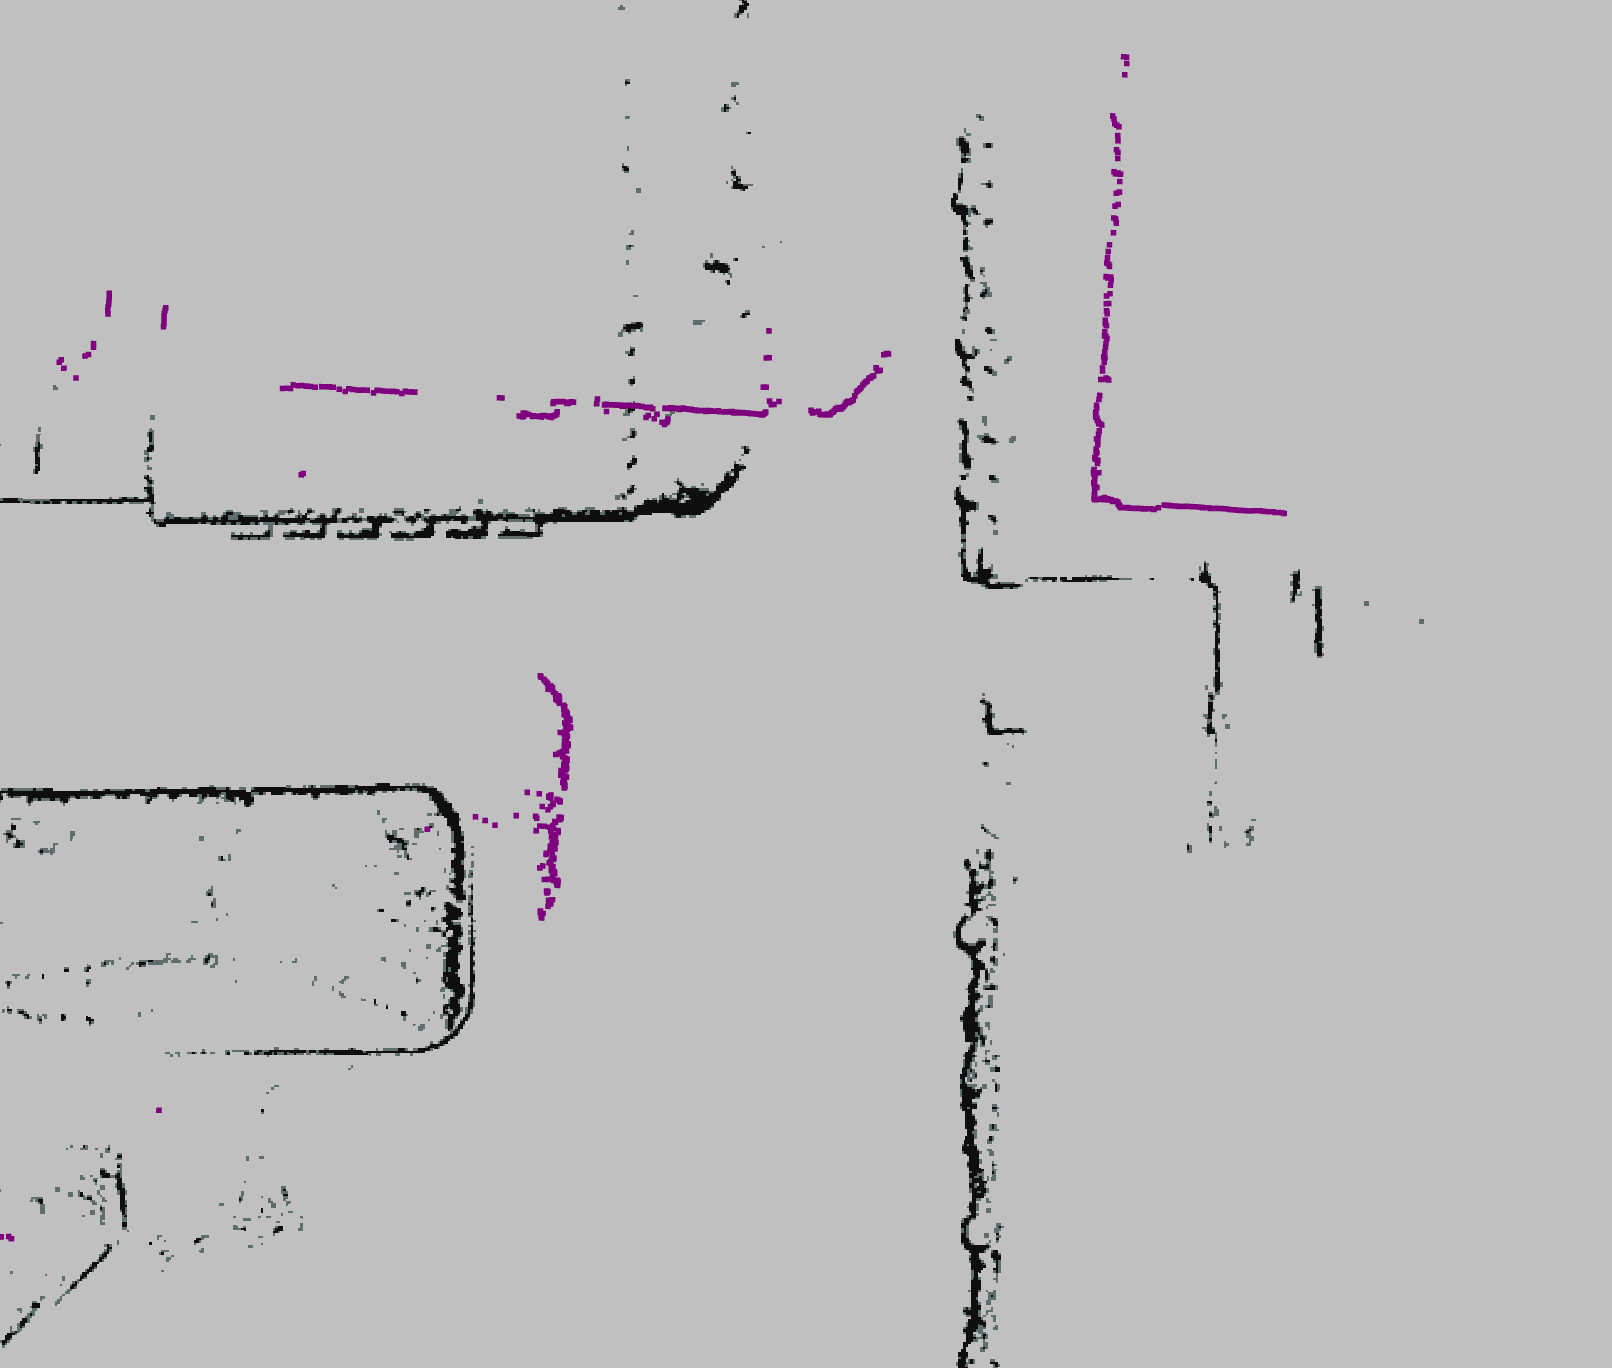
\includegraphics[height=40mm]{images/scanmap_before.png}
         \subcaption{Before AMCL adjustment}
     \end{minipage}
     \begin{minipage}[c]{65mm}
         \centering
         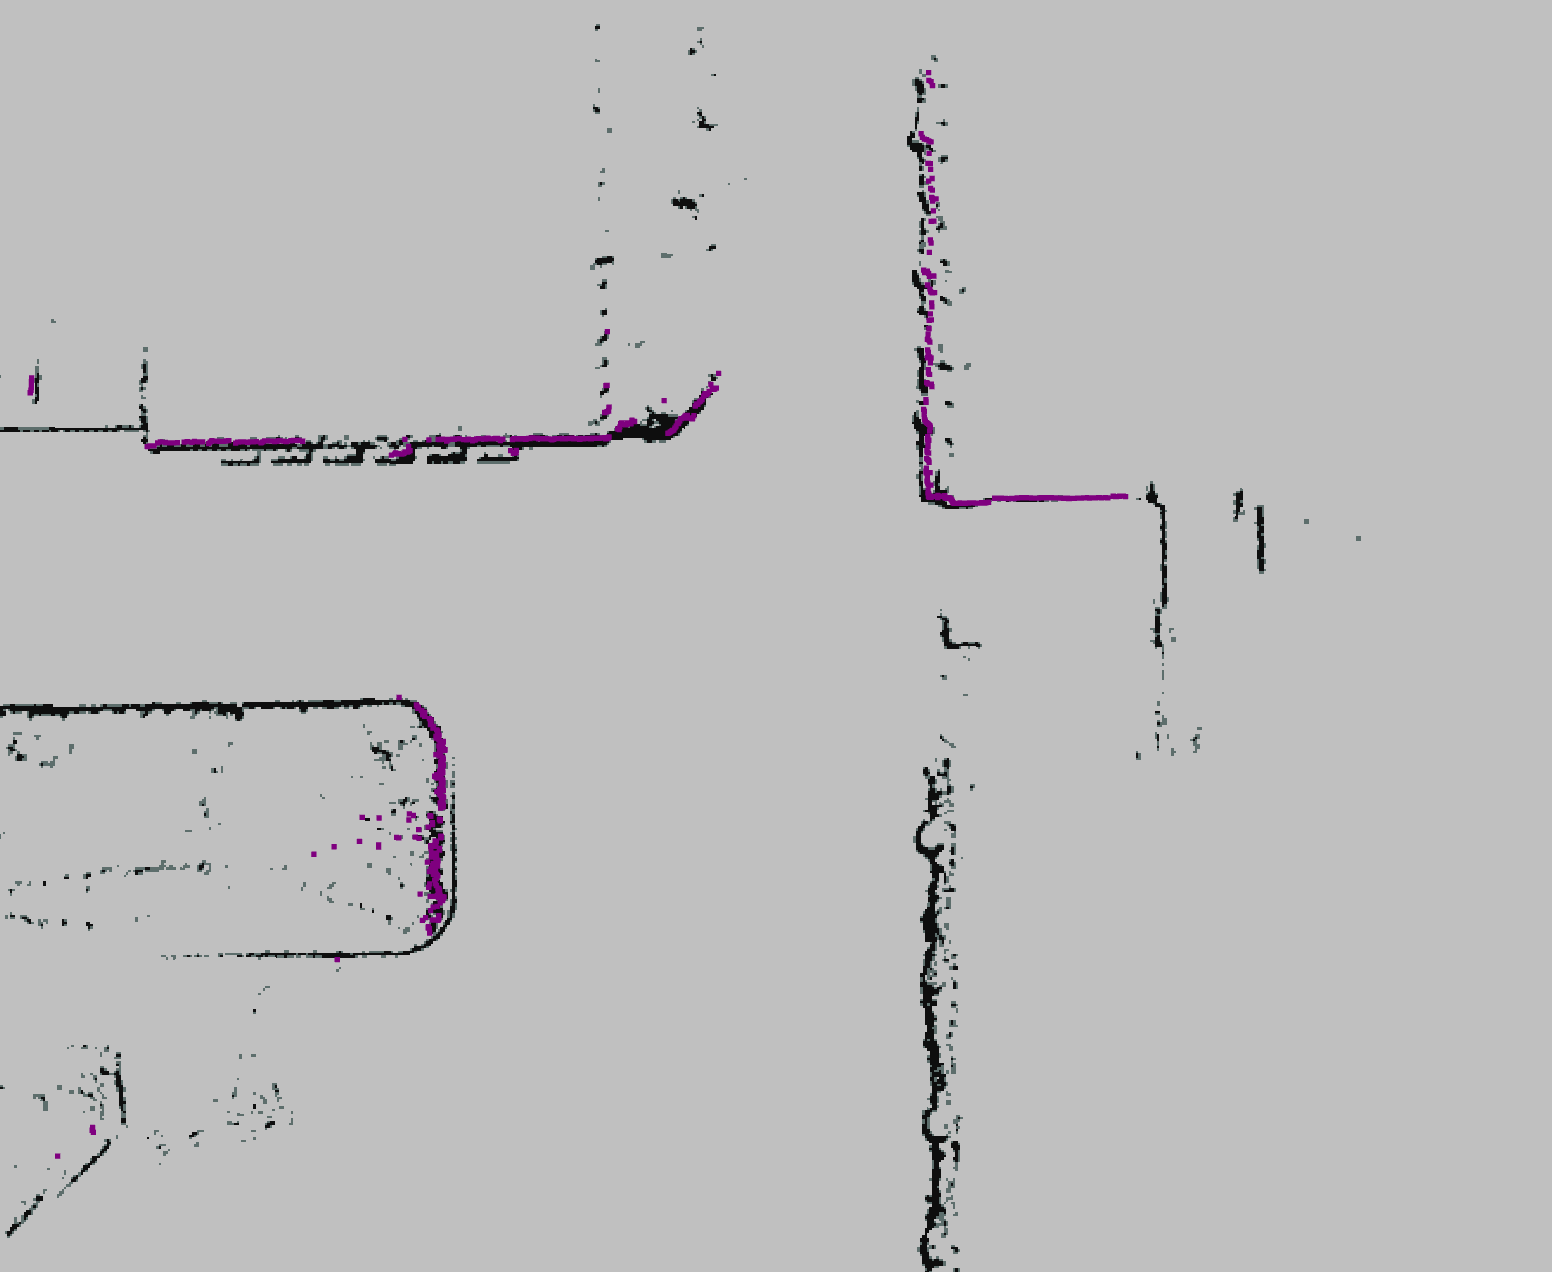
\includegraphics[height=40mm]{images/scanmap_after.png}
         \subcaption{After AMCL adjustment}
     \end{minipage}
     \caption{Map and scan visualized in Rviz}
     \label{fig:ScanandMap}
\end{figure}